
\section*{Problema P8.35}

\renewcommand*\thesection{8.35}
\numberwithin{equation}{section}

\begin{center}
    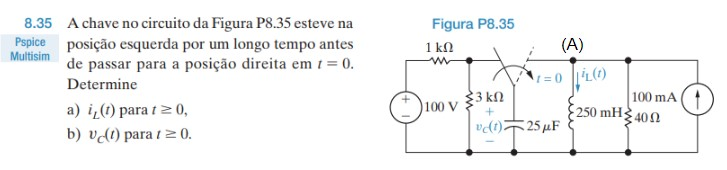
\includegraphics[scale=1.0]{P8.35.jpg}
\end{center}

O primeiro passo é entender o estado inicial do circuito para $t<0$. \\
Antes da chave comutar, o capacitor está em paralelo com um circuito divisor de tensão, e após um longo tempo possuirá tensão
inicial de 

\[ v(0) = 100\frac{3000}{1000 + 3000} \]

\begin{equation}\label{eq:8.35.1}
    v_C(0) = 75 \un{V}
\end{equation}

Além disso, o indutor se comporta como um curto-circuito para a fonte de corrente de $I = 100 \un{mA}$. Logo,  

\begin{equation}\label{eq:8.35.2}
    i_L(0) = 100 \un{mA}
\end{equation}

Exatamente no instante em que a chave comuta, em $t = 0$, temos que a corrente no capacitor é nula, pois toda a corrente
da fonte passa no indutor. Assim, temos a segunda condição inicial do capacitor 

\begin{equation}\label{eq:8.35.3}
    \diff{v(0)}{t} = 0 \un{V/s}
\end{equation}

De posse dessas condições iniciais, aplicamos análise nodal no nó essencial (A) para $t>0$, obtendo  

\[ i_c + i_L + i_R = 100 \un{mA}  \]

\[ C\diff{v_C}{t} + i_L(0) + \int_{0}^{t}v_L(t) \, dt + \frac{v_R(t)}{R} = 100 \un{mA}  \]

Usando $v_C = v_R = v_L = v(t)$,

\[ C\diff{v(t)}{t} + i_L(0) + \frac{1}{L} \int_{0}^{t}v(t) \, dt + \frac{v(t)}{R} = 100 \un{mA}  \]

Derivando ambos lados com respeito a $t$,

\[ C\diff[2]{v(t)}{t} + \frac{1}{L} v(t) + \frac{1}{R} \diff{v}{t} = 0  \]

\[ \diff[2]{v(t)}{t} + \frac{1}{RC} \diff{v}{t} + \frac{v(t)}{LC} = 0  \]

A EDO acima já possui equação característica conhecida, dada por 

\begin{equation}\label{eq:8.35.4}
    s^2 + \frac{s}{RC} + \frac{1}{LC} = 0
\end{equation}

Substituindo com os valores do enunciado,

\[ s = \frac{-(1000) \pm \sqrt{(1000)^2 - 4(1)(160000)}}{2(1)} \]

\[ s_1 = -200 \un{rad/s} \quad , \quad s_2 = -800 \un{rad/s} \]

Além disso, sabemos que a solução da EDO é da forma

\[ v(t) = Ae^{st}  \]

Com as duas raízes encontradas $s_1$ e $s_2$, temos que a solução geral é dada pela combinação linear

\begin{equation}\label{eq:8.35.5}
    v(t) = v_1(t) + v_2(t)
\end{equation}

Onde $v_1(t)$ e $v_2(t)$ são duas possíveis soluções para $v(t)$ dadas por  

\[ \begin{cases}
        v_1(t) = A_1e^{s_1t}  & \\
        \noalign{\vskip9pt}
        v_2(t) = A_2e^{s_2t}
    \end{cases}
\]

Diferenciando \eqref{eq:8.35.5} com respeito a $t$, temos duas equações

\[ \begin{cases}
        v(t) = A_1e^{s_1t} + A_2e^{s_2t} & \\
        \noalign{\vskip9pt}
        \diff{v(t)}{t} = A_1s_1e^{s_1t} + A_2s_2e^{s_2t}
    \end{cases}
\]

Em $t=0$, temos as condições iniciais já conhecidas em \eqref{eq:8.35.1} em \eqref{eq:8.35.1}

\[ \begin{cases}
        v(0) = A_1e^{s_10} + A_2e^{s_20} & \\
        \noalign{\vskip9pt}
        \diff{v(0)}{t} = A_1s_1e^{s_10} + A_2s_2e^{s_20}
    \end{cases}
    \logo
    \begin{cases}
        A_1 + A_2 = 75 \un{V} & \\
        \noalign{\vskip9pt}
        A_1s_1 + A_2s_2 = 0 \un{V/s}
    \end{cases}
\]

De posse dessas equações, temos o sistema linear para identificar os coeficientes $A_1$ e $A_2$

\begingroup
\renewcommand*{\arraystretch}{1.5}

\[
    \begin{bmatrix}
        1 & 1    \\
        s_1    & s_2
    \end{bmatrix}
    \begin{bmatrix}
        A_1 \\
        A_2
    \end{bmatrix}
    =
    \begin{bmatrix}
        75 \\
        0
    \end{bmatrix} \logo
    \begin{bmatrix}
        -s_1 & -s_1    \\
        s_1    & s_2
    \end{bmatrix}
    \begin{bmatrix}
        A_1 \\
        A_2
    \end{bmatrix}
    =
    \begin{bmatrix}
        -75s_1 \\
        0
    \end{bmatrix}
\]

\[
    \begin{bmatrix}
        -s_1 & -s_1    \\
        0    & s_2 - s_1
    \end{bmatrix}
    \begin{bmatrix}
        A_1 \\
        A_2
    \end{bmatrix}
    =
    \begin{bmatrix}
        -75s_1 \\
        -75s_1
    \end{bmatrix}
\]

\endgroup

Assim, temos  

\[ A_2 = \frac{-75s_1}{s_2 - s_1} \logo A_2 = -25\] 

\[ A_1 = 100 \] 

Conhecidos coeficientes $A_1$ e $A_2$, bem como as raízes $s_1$ e $s_2$, temos a solução geral $v(t)$ na forma de \eqref{eq:8.35.5}

\[ \boxed{v_C(t) = 100e^{-200t} - 25e^{-800t} \un{V} \, , \, t \geq 0} \]

Para encontrar $i_L(t)$, usamos a relação entre corrente e tensão no indutor   

\[ i_L(t) = i_L(0) + \frac{1}{L} \int_{0}^{t}v_C(t) \, dt \]

\[ i_L(t) = 0.1 + \frac{1}{L} \int_{0}^{t}100e^{-200t} - 25e^{-800t} \, dt \]

\[ \boxed{i_L(t) = 0.1 - 2e^{-200t} + 0.125e^{-800t} \un{A} \, , \, t \geq 0} \]



